\documentclass[11pt, oneside]{article} 
\usepackage{geometry}
\geometry{letterpaper} 
\usepackage{graphicx}
	
\usepackage{amssymb}
\usepackage{amsmath}
\usepackage{parskip}
\usepackage{color}
\usepackage{hyperref}

\graphicspath{{/Users/telliott_admin/Tex/png/}}
% \begin{center} 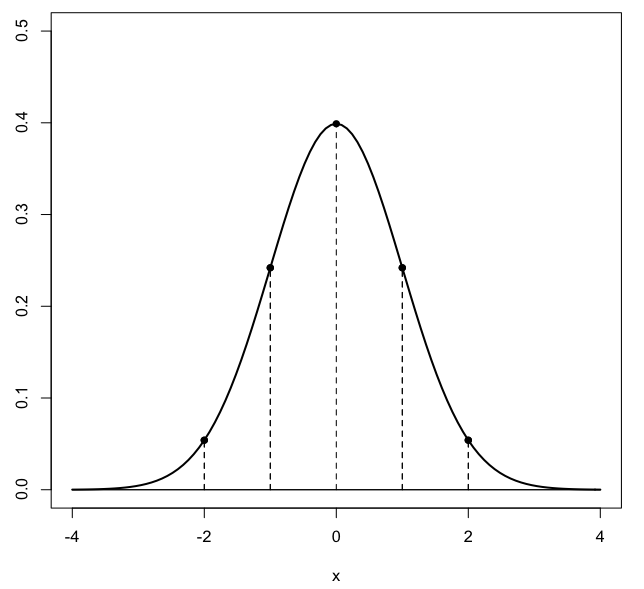
\includegraphics [scale=0.4] {gauss3.png} \end{center}

%break
\title{Between two curves}
\date{}

\begin{document}
\maketitle
\Large

By now, you should have a good handle on the integral as a measure of the area between the curve $f(x)$ and the $x$-axis.

\subsection*{below the x-axis}

One question we haven't dealt with is what happens when the curve dips below the $x$-axis.  Consider the line $y = x - 1$ which crosses the $x$-axis at $x = 1$ and the $y$-axis at $y = -1$.

\[ \int_0^1 x - 1 \ dx = \frac{x^2}{2} - x \ \bigg |_0^1 \]
\[ = \frac{1}{2} - 1 = - \frac{1}{2} \]

The absolute value of the area is correct but the sign is negative.  When we integrate a function that dips below the $x$-axis, the result will be negative.

\begin{center} 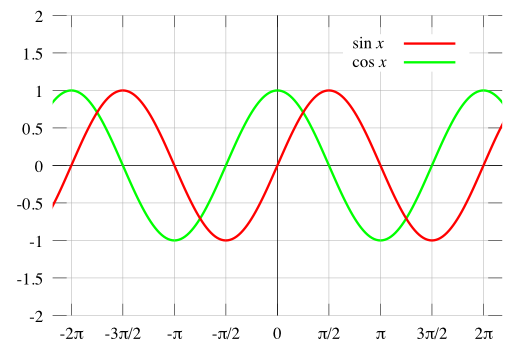
\includegraphics [scale=0.4] {sine_cosine_wikipedia.png} \end{center}

A further demonstration of this is the trigonometric functions $\sin x$ and $\cos x$:

They apparently spend as much of the time below the $x$-axis as above it.  These functions repeat with a period of $2 \pi$.  A consequence of this is that the integral of sine or cosine over a period of exactly $2 \pi$ is always equal to zero, regardless of the exact starting point.

\[ \int_0^{2\pi} \sin x \ dx = - \cos x \ \bigg |_0^{2\pi} = - (-1) - 1 = 0 \]

This is true for \emph{any} bounds whose difference is $2 \pi$.

\subsection*{two curves}
A common application of integrals is to give the area between two curves, which is obtained simply by subtracting one function from another and integrating the difference.

\[ A = \int f(x) - g(x) \ dx \]

\subsection*{an easy problem}
Consider the two curves $y = \sqrt{x}$ and $y = x^2$.  These curves cross at
\[ \sqrt{x} = x^2 \]
We can see by inspection that this happens at $x = 0$ and $x = 1$.

In this region ($0 \le x \le 1$) the square root is larger than the square.

Furthermore, we already calculated that the part below $y = x^2$ is $1/3$ of the area of the rectangle with corners $(0,0)$ and $(x,y)$.  The same is true for the area above the square root.  From this we can predict what the result will be.

\[ A = \int f(x) - g(x) \ dx \]
For this problem
\[ A = \int_0^1 \sqrt{x} - x^2 \ dx \]
\[ = \frac{2}{3} x^{3/2} - \frac{x^3}{3} \ \bigg |_0^1  \]
\[ = \frac{2}{3} - \frac{1}{3} = \frac{1}{3} \]

\subsection*{a more complicated problem}
Consider the two curves $y = x$ and the unit circle $y = \sqrt{1 - x^2}$.
\begin{center} 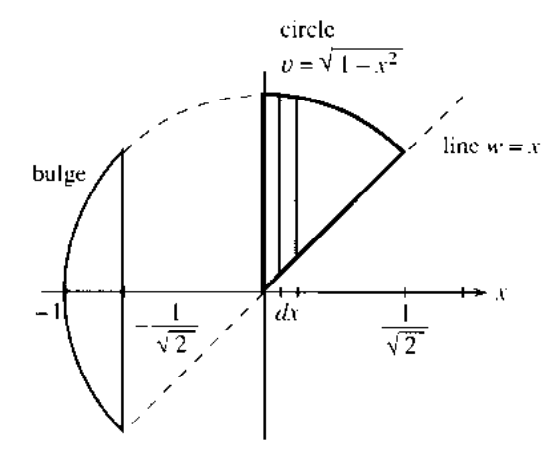
\includegraphics [scale=0.4] {between_curves.png} \end{center}
We see that the circle lies above the line for most of its length.  However, it's complicated.  Part of the figure is below the $x$-axis, and there is a bulge on the left end.

The key is that we must appreciate the relationship (know which is on top) in order to do integrals of differences between curves properly.

First solve for the points where the two curves cross:
\[ y = x = \sqrt{1 - x^2} \]
\[ 2x^2 = 1 \]
\[ x = \pm \sqrt{1/2}\ = \pm \frac{1}{\sqrt{2}} \]
\[ y = \pm \frac{1}{\sqrt{2}} \]

The area of the sector in the first quadrant is pretty easy.
\[ A = \int_0^{1/\sqrt{2}} \sqrt{1 - x^2}  - x \ dx \]
\begin{center} 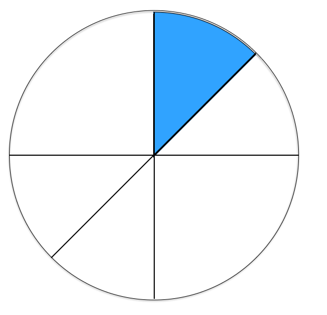
\includegraphics [scale=0.4] {between_curves2.png} \end{center}

We solved $\int \sqrt{1 - x^2} \ dx$ in the previous chapter:
\[ = \frac{1}{2} \ [ \ \sin^{-1} x + x \sqrt{1-x^2} \ ] \ - \frac{x^2}{2} \ \bigg |_0^{1/ \sqrt{2}} \]
At the lower bound everything including $\sin^{-1} x$ is zero, and at the upper bound we have
\[ =  \frac{1}{2} \ [ \ \frac{\pi}{4} + \frac{1}{\sqrt{2}} \ \frac{1}{\sqrt{2}} \ ] - \frac{1}{4} = \frac{\pi}{8} \]
which we confirm from elementary geometry is just a slice of the pie.

For the area to the left of the $y$-axis we must think a little more.  The line $y=x$ dips below the $x$-axis, so the integral of the second part $g(x)$
\[ \int_{-1/\sqrt{2}}^0 x \ dx \]
is negative.

It's probably less confusing to just do the parts above and below the $x$-axis separately!

\begin{center} 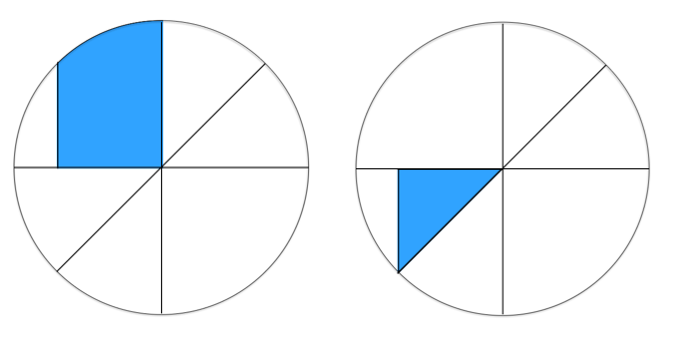
\includegraphics [scale=0.4] {between_curves3.png} \end{center}

The area above the $x$-axis is
\[ A = \frac{1}{2} \ [ \ \sin^{-1} x + x \sqrt{1-x^2} \ ] \ \bigg |_{-1/ \sqrt{2}}^0 \]
At the upper bound, we have again zero, and at the lower bound
\[ \frac{1}{2} \ [ \ - \frac{\pi}{4} + (-\frac{1}{\sqrt{2}}) \ \frac{1}{\sqrt{2}} \ ] \]
which must be subtracted, so we change signs and obtain
\[ \frac{\pi}{8} + \frac{1}{4} \]

For the area below the $x$-axis:
\[ \int_{-1/ \sqrt{2}}^0 x \ dx \]
\[ = \frac{x^2}{2} \ \bigg |_{-1/ \sqrt{2}}^0 = - \frac{1}{4} \]
The area below the $x$-axis is \emph{minus} the result of the integral (the integral yields a negative area).

So lose the minus sign
\[ A = \frac{1}{4} \]

The total for this region (between $- 1/\sqrt{2}$ and $0$) is then just
\[ \frac{\pi}{8} + \frac{1}{4} + \frac{1}{4} = \frac{\pi}{8} + \frac{1}{2} \]
This is effectively a slice of pie plus a triangle of base $2/\sqrt{2}$ and height $1/\sqrt{2}$.

The third part is the bulge to the left of $x = - 1/\sqrt{2}$.  

\begin{center} 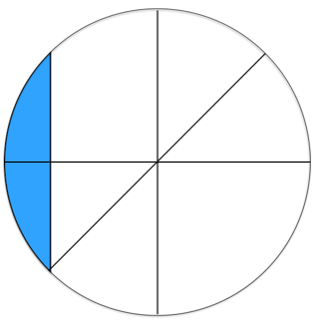
\includegraphics [scale=0.4] {between_curves4.png} \end{center}

We will calculate the area above the $x$-axis and multiply by two:
\[ A = 2 \int_{-1}^{-1/\sqrt{2}} \sqrt{1 - x^2} \ dx \]
\[ = 2 \ \frac{1}{2} \ [ \ \sin^{-1} x + x \sqrt{1-x^2} \ ]  \ \bigg |_{-1}^{-1/ \sqrt{2}} \]
The leading factors cancel.
\[ =  \sin^{-1} x + x \sqrt{1-x^2} \ ]  \ \bigg |_{-1}^{-1/ \sqrt{2}} \]

At the upper bound we have (as we found before)
\[ = - \frac{\pi}{4} - \frac{1}{\sqrt{2}} \ \frac{1}{\sqrt{2}}  = - \frac{\pi}{4} - \frac{1}{2} \]
At the lower bound, $\sin^{-1} x = - \pi/2$ and $x \sqrt{1-x^2}$ is zero.  

We're subtracting, so we have
\[ = - \frac{\pi}{4} - \frac{1}{2} + \frac{\pi}{2} \]
\[ = \frac{\pi}{4} - \frac{1}{2} \]

Adding all the pieces together
\[ A = \frac{\pi}{8} + \frac{\pi}{8}  + \frac{1}{2} + \frac{\pi}{4}  - \frac{1}{2} =  \frac{\pi}{2}  \]
which is obviously correct.

\end{document}